% Fig. 4.13 -- 取倒數之後右尾機率變成左尾機率 (兩面板加箭頭)。
% 書稿來源: mathstatch4.tex 第 4915 至 4947 行 (左面板) 與第 4950 至 4982 行 (右面板)，
%   兩個 tikzpicture 同在一個 tabular 的第一欄與第三欄，中間第二欄是
%   $\xRightarrow[]{~1/F~}$。依 CH4_FIGURE_SPECS.md 第 3.2 節，網頁把箭頭一併畫進圖內。
%
% 密度: F(d1,d2) 的 pdf 寫成單一個 exp，
%   f(x) = exp( lnC + (d1/2-1) ln x - ((d1+d2)/2) ln(1 + (d1/d2) x) )，
%   lnC = lgamma((d1+d2)/2) - lgamma(d1/2) - lgamma(d2/2) + (d1/2) ln(d1/d2)。
%   左面板 F(10,50): lnC = 5.247066 (即 C = 190.008)。
%   右面板 F(50,10): lnC = 53.530204。
%   寫成單一個 exp 是必要的: 若拆成 190.008*x^4*(1+0.2x)^(-30)，x 接近 3 時中間值達
%   15390，逼近 pgfmath 的 16384 上限，而 (1+0.2x)^(-30) 又落在 pgfmath 的 1e-5 解析度
%   之下，兩端都會失真。
%
% 對書稿原圖的一處刻意改正 (依 SITE_STYLE_CANON.md 第〇節第 5 點，另行登錄勘誤):
%   書稿右面板的界點寫 0.379201，但 0.379201 是 F_{0.95}(10,50)，不是 F_{0.95}(50,10)，
%   自由度沒有跟著對調。實際數字為
%     F_{0.05}(10,50) = 2.0261430   (左面板的界點，右尾機率恰為 0.05)
%     1/2.0261430     = 0.4935486 = F_{0.95}(50,10)   (右面板應有的界點)
%     0.379201        = 1/F_{0.05}(50,10) = 1/2.6371240 = F_{0.95}(10,50)
%   以書稿的 0.379201 作圖，右面板填色的左尾機率只有 0.0116，與左面板的 0.05 對不上，
%   而本圖要講的正是兩塊尾機率相等、兩個界點互為倒數，故網頁採 0.4935486。
%   該點的密度為 0.4857167 (書稿在 0.379201 處記 0.1935353，數值本身無誤)。
%
% 版面: x = 1.15cm、y = 2.944cm，兩者之比保住書稿 height = 0.8 x width 的比例
%   (x 範圍 3.2、y 範圍 1)。左面板原點在 0，右面板原點在 5.0 (x 單位)，中間留給箭頭。
%   兩面板的座標範圍完全相同，讀者才看得出 2.0261430 與 0.4935486 互為倒數。
%
% 字級: 全圖標示一律 \large (12pt)，\DeclareMathSizes{12}{12}{10}{9} 把 script 級撐到
%   10pt。圖內最小的一級是 F 的下標 alpha 與 1-alpha，即 10pt；沒有 scriptscript。
%   原生尺寸 282.826 x 106.327 pt。S pt 的字在顯示寬 W 之下為 S x 0.99626 x W / 282.826
%   px，故 topic-figure--wide 在手機 350 px 之下 12pt 為 14.80px、10pt 為 12.33px，
%   桌面 620 px 之下為 26.22 / 21.85px。本圖落在 topic-proof 之內，該處手機的可用寬度
%   約 330 px，10pt 仍有 11.62px，守住 11px 的下限。
%   覆核: 由 SVG 的墨跡高度反算，數字 1 在 script 級為 6.5938pt、在 12pt 為 7.8906pt，
%   比值 0.835，即 10/12，可知 \DeclareMathSizes 確實生效 (未宣告時為 8.5/12 = 0.708)。
%
% 標示間距 (CH2_FIGURE_SPECS.md 1.3 要求相鄰標示至少 0.6cm):
%   左面板 0 與 F_alpha(10, 50) 相距 1.254cm；左面板該標示與右面板 F_{1-alpha}(50, 10)
%   相距 1.817cm。兩個曲線標示都在該處曲線高度的三倍以上，不相碰。
\documentclass[tikz,border=2pt]{standalone}
\usepackage{amsmath}
\usepackage{amssymb}
\usepackage{xcolor}
\usetikzlibrary{arrows.meta}
\DeclareMathSizes{12}{12}{10}{9}

\definecolor{journalink}{HTML}{1F1C18}
\definecolor{journalmuted}{HTML}{8A7F72}
\definecolor{journalaccent}{HTML}{9C2D2D}

\begin{document}
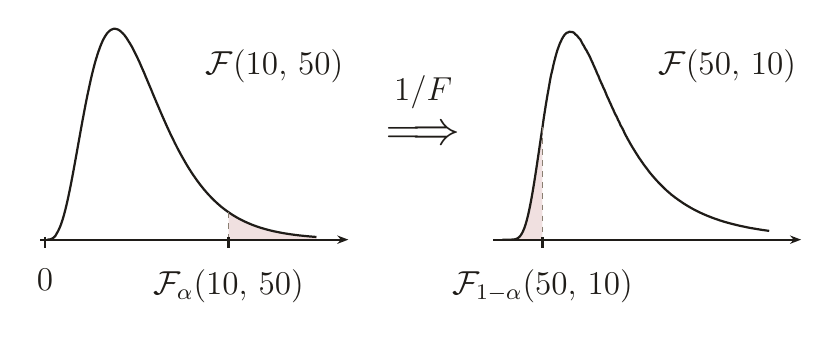
\begin{tikzpicture}[
  x=1.15cm,
  y=2.944cm,
  every node/.style={font=\large, journalink},
  axis/.style={journalink, line width=0.8pt, -{Stealth[length=4pt]}},
  tick/.style={journalink, line width=0.8pt},
  curve/.style={journalink, line width=0.8pt},
  guide/.style={journalmuted, line width=0.5pt, dash pattern=on 2pt off 2pt},
  region/.style={journalaccent, fill opacity=0.15}
]

  %% ---- 左面板: F(10,50)，填右尾 --------------------------------------
  \begin{scope}[shift={(0,0)}]
    \fill[region]
      (2.0261430,0) -- (3,0) -- (3,0.0115786)
      -- plot[domain=3:2.0261430, samples=120, smooth]
         (\x,{exp(5.247066+4*ln(\x)-30*ln(1+0.2*\x))})
      -- cycle;

    \draw[curve] plot[domain=0.02:3, samples=220, smooth]
      (\x,{exp(5.247066+4*ln(\x)-30*ln(1+0.2*\x))});

    \draw[axis] (-0.05,0) -- (3.35,0);

    \draw[guide] (2.0261430,0.1183158) -- (2.0261430,0);
    \foreach \p in {0, 2.0261430}
      \draw[tick] ([yshift=0.035cm]\p,0) -- ([yshift=-0.106cm]\p,0);
    \node[anchor=north] at ([yshift=-0.25cm]0,0) {$0$};
    \node[anchor=north] at ([yshift=-0.25cm]2.0261430,0)
      {$\mathcal{F}_{\alpha}(10{,}~50)$};

    \node[anchor=east, inner sep=0pt] at (3.30,0.75)
      {$\mathcal{F}(10{,}~50)$};
  \end{scope}

  %% ---- 中間的箭頭 -----------------------------------------------------
  \node[inner sep=0pt, font=\LARGE] at (4.175,0.45) {$\Longrightarrow$};
  \node[anchor=south, inner sep=0pt] at (4.175,0.56) {$1/F$};

  %% ---- 右面板: F(50,10)，填左尾 --------------------------------------
  \begin{scope}[shift={(5.0,0)}]
    \fill[region]
      (0,0) -- (0.4935486,0) -- (0.4935486,0.4857167)
      -- plot[domain=0.4935486:0.05, samples=120, smooth]
         (\x,{exp(53.530204+24*ln(\x)-30*ln(1+5*\x))})
      -- cycle;

    \draw[curve] plot[domain=0.05:3, samples=220, smooth]
      (\x,{exp(53.530204+24*ln(\x)-30*ln(1+5*\x))});

    \draw[axis] (-0.05,0) -- (3.35,0);

    \draw[guide] (0.4935486,0.4857167) -- (0.4935486,0);
    \draw[tick] ([yshift=0.035cm]0.4935486,0) -- ([yshift=-0.106cm]0.4935486,0);
    \node[anchor=north] at ([yshift=-0.25cm]0.4935486,0)
      {$\mathcal{F}_{1-\alpha}(50{,}~10)$};

    \node[anchor=east, inner sep=0pt] at (3.30,0.75)
      {$\mathcal{F}(50{,}~10)$};
  \end{scope}

\end{tikzpicture}
\end{document}
